\documentclass[aps,twocolumn,twoside,secnumarabic,balancelastpage,amsmath,amssymb,nofootinbib,hyperref=pdftex]{revtex4}


\usepackage{color}         % produces boxes or entire pages with colored backgrounds
\usepackage{graphics}      % standard graphics specifications
\usepackage[pdftex]{graphicx}      % alternative graphics specifications
\usepackage{longtable}     % helps with long table options
\usepackage[english]{babel}
\setlength{\parskip}{1em}
\usepackage{amsmath}
\usepackage{epsf}          % old package handles encapsulated post script issues
\usepackage{bm}            % special 'bold-math' package
\usepackage{verbatim}			% for comment environment
\usepackage[colorlinks=true]{hyperref}  % this package should be added after all others % use as follows: \url{http://web.mit.edu/8.13}                   
\renewcommand{\thesection}{\Roman{section}}                                  

\begin{document}
\title{Modified Minimal Flavor Violation and Nucleon Decay}
\author         {Noah Steinberg, James D. Wells, Zhengkang Zhang}
%\email          {nastein@umich.edu}
%\date{\today}
\affiliation{Leinweber Center for Theoretical Physics, University of Michigan, Ann Arbor, MI 48104, USA}

\begin{abstract}
\small{We study nucleon decay under several versions of Modified Minimal Flavor Violation (MMFV). These MMFV scenarios arise in many Grand Unified Theories which unite quarks and leptons into the same multiplets, leading to a smaller flavor symmetry group than the SM. Dominant decay modes are identified in each case, bounds on Wilson coefficients and the baryon number violating scale, and relationships between different nucleon decay observables are uncovered.}
\end{abstract}

\maketitle

\section{Introduction}
Baryon number conservation, first formulated by Hermann Weyl in 1929\cite{Weyl}, is expected to be violated by many beyond the Standard Model (BSM) theories. As an accidental global symmetry of the SM, there is no fundamental reason to expect this symmetry to be exact. Indeed, according to common folklore in quantum gravity, the only good global symmetry is a broken one\cite{QG}. Nucleon decay is an observable consequence of baryon number violation (BNV), but extensive searches have placed the lower lifetime limit of proton decay at $\tau_{p}\approx 10^{33-34}$ years\cite{SuperK}. Whatever the mechanism responsible for BNV, these experimental constraints require the scale of BNV interactions to be many orders of magnitude larger than the weak scale. This separation of scales enables an EFT approach to nucleon decay.

In the Standard Model Effective Field theory (SMEFT) there are 4 baryon number violating operators\cite{Weinberg} at lowest dimension, d = 6;

\begin{equation}  \label{eq:1}
  \begin{aligned}
  Q^{duql}_{prst} &= \frac{C^{prst}_{duql}}{\Lambda^2}(\bar{d}^{c}_{p}u_{r})(\bar{q}^{ci}_{s}l^{j}_{t})\epsilon_{ij} \\
  Q^{qque}_{prst} &=  \frac{C^{prst}_{qque}}{\Lambda^2}(\bar{q}^{ci}_{p}q^{j}_{r})(\bar{u}^{c}_{s}e_{t})\epsilon_{ij} \\
  Q^{qqql}_{prst} &=  \frac{C^{prst}_{qqql}}{\Lambda^2}(\bar{q}^{ci}_{p}q^{j}_{r})(\bar{q}^{ck}_{s}l^{l}_{t})\epsilon_{il}\epsilon_{jk} \\
  Q^{duue}_{prst} &=  \frac{C^{prst}_{duue}}{\Lambda^2}(\bar{d}^{c}_{p}u_{r})(\bar{u}^{c}_{s}e_{t}),
  \end{aligned}
\end{equation}

where all fields are Dirac spinors, c refers to the charge conjugated operator, p,r,s, and t are generation indices,
 q and l are left handed quark and lepton SU(2) doublets with appropriate indices i,j,k,l, and u, d, and e are up, down quark and lepton SU(2) singlets. Each operator is understood to be antisymmetrized in color. We have explicitly written out the Wilson coefficients and an overall scale $\frac{1}{\Lambda^2}$, with $\Lambda$ being the scale of BNV interactions. 

Given a specific BSM theory, one computes the combination $\frac{C^{prst}}{\Lambda^2}$ for each of the dimension 6 operators in Eqn. \ref{eq:1} by integrating out heavier fields such as the SU(5) X and Y gauge bosons, or the heavy triplet Higgs fields, and then computes nucleon lifetimes. In this way, the parameter space of each BSM theory can be constrained by existing nucleon lifetime measurements. In the absence of a specific BSM theory, what can one say about the the Wilson coefficients, while remaining as agnostic as possible? A key observation is that the Wilson coefficients contain all the information about the flavor structure of the BNV operators in Eqn. \ref{eq:1}. Flavor symmetries then can constrain the types of flavor changing nucleon decays which are possible, as well as give us a hint at the relative levels of suppression of different decay channels. This scenario is usually approaching through the assumption of Minimal Flavor Violation (MFV). 

The SM is invariant under the flavor group $G^{\text{SM}}_{f} = SU(3)^{5}_{\text{flavor}}$, where one copy of $SU(3)_{\text{flavor}}$\footnote{The flavor subscript distinguishes these $SU(3)$ from $SU(3)_{\text{color}}$} corresponds to the q,l,u,d, and e fields respectively. This symmetry is broken only by the Yukawa coupling of the Higgs to the fermions. MFV is the assumption that whatever the UV theory is, its flavor structure is entirely dictated by the SM Yukawa couplings. In essence the CKM matrix determines the strength of any flavor changing effects in the standard model and beyond. To implement MFV, one promotes the SM Yukawa couplings to spurions, which transform appropriately under  $G^{\text{SM}}_{f}$ so as to restore flavor symmetry. Then for any new operators, one inserts linear combinations of powers of the Yukawas so as to make the operators invariant under  $G^{\text{SM}}_{f}$. This generally produces a series of the form:

\begin{equation}
a_{0}1 + a_{1}Y_{u}Y^{\dagger}_{u} + a_{2}Y_{u}Y_{d} + . . . . 
\end{equation}
where the $a_{i}$ are $\mathcal{O}(1)$ coefficients.

Next the Yukawas are frozen to their physical values by choosing, for example, $Y_{u}=\text{diag}(\lambda_{u},\lambda_{c}, \lambda_{t})$ and $Y_{d}=V_{\text{CKM}}\text{diag}(\lambda_{d},\lambda_{s}, \lambda_{b})$. Operators with more insertions are then suppressed by powers of Yukawa couplings and CKM elements. For a more thorough review see \cite{MFV}. The issue with the dimension 6 BNV operators is that they cannot be made invariant under the SM flavor group\cite{dim6nogo}. Thus traditional MFV cannot tell us the flavor structure of the Wilson coefficients $C^{prst}_{i}$. 

Given this, all hope is not lost. It is likely that in a Grand Unified Theory (GUT), which combines certain quarks and leptons of the same generation into the one multiplet, that the flavor symmetry group is much smaller than in the SM. With a smaller flavor symmetry group it may be possible that the BNV operators of Eqn. \ref{eq:1} can be made into flavor singlets, and thus the flavor structure of these operators illuminated. This will be the content of this paper. 

\section{Modified Minimal Flavor Violation}

\subsection{$G^{(2)}_{f}$}

We begin with an example of MMFV, where the flavor symmetry group is $G^{(2)}_{f} = SU(3)^{2}_{\text{flavor}}$. Under this group the fermions transform as:

\begin{equation}
 \begin{aligned}
 l, d^{c}&(\bold{3},1) \\
 q,u^{c}, e^{c}&(1,\bold{3}).
 \end{aligned}
\end{equation}

The SM, minus Yukawa interactions, is obviously invariant under $G^{(2)}_{f}$ because it is a subgroup of $G^{SM}_{f}$. We can include Yukawa interactions by promoting the Yukawa couplings to spurions transforming as:

\begin{equation}
 \begin{aligned}
Y_{u}&(\bold{\bar{6}},1)\\
Y_{d},Y^{T}_{e}&(\bold{\bar{3}},\bold{\bar{3}})
 \end{aligned}
\end{equation}

Examining our BNV operators in Eqn. \ref{eq:1} and working to lowest order in the Yukawa couplings, we see that these operators can be made invariant under $G^{(2)}_{f}$ if the Wilson coefficients have the following structure:

\begin{equation} \label{eq:5}
 \begin{aligned}
 C^{prst}_{qqql} &= Y^{pr}_{u}Y^{st}_{d} + Y^{ps}_{u}Y^{rt}_{d} + Y^{rs}_{u}Y^{pt}_{d}\\
 C^{prst}_{duql} &= \delta^{pt}\delta^{rs}\\
 C^{prst}_{qque} &= \delta^{ps}\delta^{rt} + \delta^{rs}\delta^{pt}\\
 C^{prst}_{duue} &= (Y^{\dagger}_{d})^{pr}(Y^{\dagger}_{u})^{st} + (Y^{\dagger}_{d})^{ps}(Y^{\dagger}_{u})^{rt}
 \end{aligned}
\end{equation}

In the above it is understood that there is an $\mathcal{O}(1)$ coefficient in front of each term. Notice that $C_{duql}$ and $C_{qque}$ require no insertions of Yukawa matrices to make their corresponding operators flavor singlets. Thus, these operators will give the dominant contribution to nucleon decay. Additionally, once the Wilson coefficients of Eqn. \ref{eq:5} are inserted into Eqn. \ref{eq:1}, we have totally fixed the flavor structure of the operators. This is what makes MMFV a very powerful organizing principle.

Below the EW symmetry breaking scale $\mathcal{O}_{duql}$ produces a single operator, $c(\bar{s}^{c}_{R}u_{R})(\bar{d}^{c}_{L}\nu_{\mu L})$, where c is an overall Wilson coefficient evaluated at the EW breaking scale, which contributes to $P\rightarrow K^{+}\bar{\nu}$, a highly sought after proton decay channel which is favored by many SUSY GUT theories. The proton lifetime/Branching Ratio can be calculated in terms of the Wilson coefficient evaluated at $\mu = M_{\text{Z}}$, multiplied by a long range renormalization factor to run the coefficient down to 2 GeV where the nucleon matrix elements are calculated using lattice QCD\cite{lattice}. Figure \ref{fig:1} shows the proton lifetime/Branching Ratio for $P\rightarrow K^{+}\bar{\nu}$ as a function of the overall coefficient mentioned above and the BNV scale $\Lambda$. 

\begin{figure}[htbp]
\begin{center}
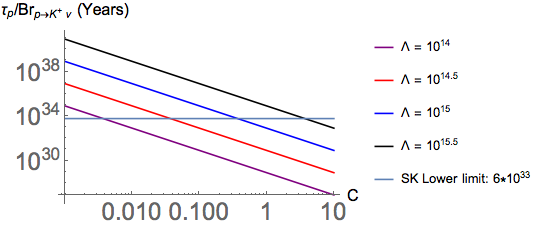
\includegraphics[width=9cm]{fig1.png}
\caption{Proton Lifetime/Branching Ratio in the $G^{(2)}_{f}$ flavor symmetry scenario for $P\rightarrow K^{+}\bar{\nu}$  vs overall Wilson coefficient for several values of BNV scale $\Lambda$.}
\label{fig:1}
\end{center}
\end{figure}

\subsection{$G^{(3)}_{f}$}

In this example, the flavor symmetry group is $G^{(3)}_{f} = SU(3)_{\text{flavor}}^{3}$ with the fermions transforming as:

\begin{equation}
 \begin{aligned}
 l, u^{c}&(\bold{3},1,1) \\
 q,d^{c}&(1,\bold{3},1) \\
 e^{c}&(1,1,\bold{3}).
 \end{aligned}
\end{equation}

Again we can identify the dominant BNV contribution by looking at which operators from Eqn. \ref{eq:1} can be made into flavor singlets with no Yukawa insertions. Clearly only $\mathcal{O}_{duql}$ satisfies this requirement.

\subsection{$G^{(1)}_{f}$}

\begin{thebibliography}{9} 

\bibitem{Weyl} H. Weyl, Z. Phys. 56, 330 (1929) [Surveys High Energ. Phys. 5, 261 (1986)].

\bibitem{QG} Kallosh, R. Linde, A. Linde, L. Dmitri, L. Susskind. Phys. Rev. D. 52. 10.1103 (1995).

\bibitem{SuperK}  S. Mine and Super Kamiokande Collaboration 2016 J. Phys.: Conf. Ser. 718
062044

\bibitem{Weinberg} S. Weinberg, Phys. Rev. Lett. 43, 21 (1979).

\bibitem{MFV} G. Isidori, D. M. Straub. The European Physical Journal C. 72, 8 (2012).

\bibitem{dim6nogo}  R. Alonso et al. JHEP 1404 (2014) 159 arXiv:1312.2014 [hep-ph] CERN-PH-TH-2013-305

\bibitem{lattice} Y. Aoki et al., Phys. Rev. D 96, no. 1, 014506 (2017)

\end{thebibliography}









\end{document}